\documentclass[12pt]{article}
\usepackage{geometry}
 \usepackage{graphicx}
 \usepackage{multirow}
\usepackage{fancyvrb}
\usepackage{float}
\graphicspath{{figs/}}     
\usepackage{titlesec}
\usepackage[colorlinks=true]{hyperref}
\geometry{a4paper} % or letter or a5paper or ... etc
% \geometry{landscape} % rotated page geometry

% See the ``Article customise'' template for come common customisations

\title{CSE380 Final Project: Finite Element Solution of the Steady Heat Equation}
\author{Christopher Cameron}
\date{} % delete this line to display the current date

%%% BEGIN DOCUMENT
\begin{document}

\maketitle

\section*{Project Overview}
\subsection*{Motivation and Goals}

As an experimentalist I have had little exposure to serious computational science and coding development.  I have data processing routines, and some small reduced order models implemented in matlab, but my experience with compiled code is limited to small modifications to large codes for class projects.  My goal for this project, and for this entire course, was to gain the largest exposure possible to the process and tools involved in writing scientific codes while also learning about coding techniques themselves.

To this end I chose a simple project, solving the steady heat equation, which would allow me to build an application from scratch.  I chose to implement my solution using the finite element for two reasons.  The first is that I am familiar with the techniques involved from my coursework and some research scripts I have written.  The second is that the finite element method inherently lends itself to an object oriented program methodology.  My past coding experience was limited to procedural coding and I wanted to use C++ and attempt to expose myself to a new way of tackling problems that is more modular and flexible.

The end result is a 1d steady heat equation solver which could be expanded to 2d dimension or unsteady problems fairly rapidly.  Eigen is used for assembling and solving the matrix equations, while grvy is used for input parsing and timing.  Verification was accomplished through a combination of unit tests implemented with the Catch library and manufactured solution based verification with the MASA library \cite{MASA}.  A github repository was created which was very useful, especially when stampede was down and I needed a branch of my code that didn't include grvy due to compilation issues on my local machine.

\subsection*{The Steady Heat Equation and Finite Element Method}

The steady heat equation shown in equation \ref{eq:heat} is an elliptic PDE, which simplifies in one dimension to the differential equation given by equation \ref{eq:heat1d}.  To formulate the finite element problem we cast the equation into variational form, multiplying by a test function v and integrating over the problem domain.  In particular for the galerkin finite element method the test and trial functions are chosen from the same space.  The overall functions are composed of the summation of functions with limited support on the solution domain, allowing all integrations to be performed locally on what are known as elements.

\begin{equation}
\label{eq:heat}
   -\nabla \cdot \left(k(x,y)\nabla u(x,y) \right) = f(x,y)\\
\end{equation} 

\begin{equation}
\label{eq:heat1d}
    -\frac{d}{dx}\left(k(x)\frac{du}{dx}\right) = f(x) 
\end{equation} 

\begin{equation}
\label{eq:fe}
 \sum_{i = 1}^n\sum_{j = 1}^n \int_a^b k(x)\frac{du_i}{dx}\frac{dv_j}{dx}\,dx. = \sum_{i = 1}^n\int_a^b f(x)u_i\,dx.
\end{equation}

Equation \ref{eq:fe} shows the variational formulation of the problem with test and trial function that are a summation of these limited support functions.  The test and trial functions are comprised of a shape function $\phi_i$ multiplied by an unknown weight $a_i$.  Performing the element-wise integrations in \ref{eq:heat_1dfe} results in a linear system of equations Ax = b, where the vector x is the unknown weights $a_i$.  For this problem 1st and 2nd order Lagrangian shape functions were chosen, shown in figure \ref{fig:shape}

\begin{figure}[!htbp] 
   \centering
\label{fig:shape}
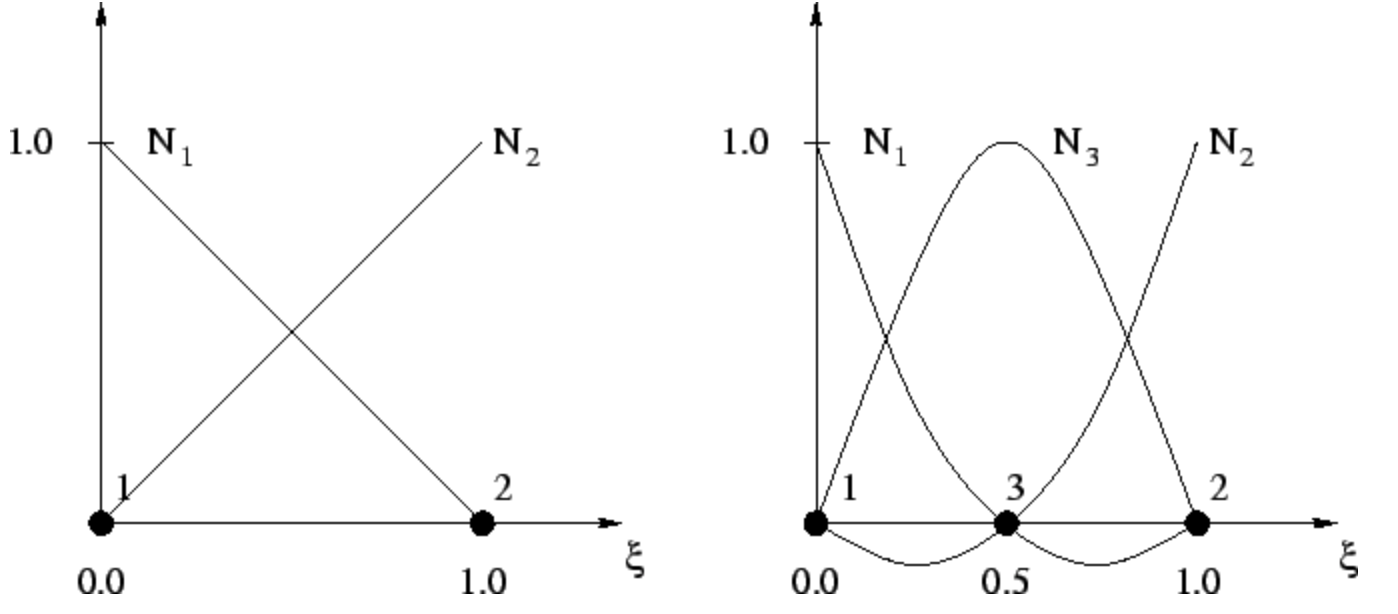
\includegraphics[height = 5cm]{shapes.png}
\caption{1st and 2nd order Lagrangian shape functions \cite{radi_shape_func}}
\end{figure}

Once the system of equations is assembled the linear system is solved for the unknown weights and the solution computed by summing the contributions of all shape functions multiplied by their corresponding weights.

\section*{Implementation}

The finite element method naturally lends itself to an object oriented programming style, as the solution involves discretizing the domain into elements with edges and nodes, discrete objects each with a set of properties.  The actual construction of the solution also involves several steps which are really local operations on elements or lines, which translate into object methods.  The program structure was first written out on paper, then implemented in a Matlab code which reused some legacy routines available from earlier coursework.  Before the C++ programming began the structure was set such that objects would be created for the following: The problem domain, the elements, the edges, the nodes, and the solver.

\subsection*{Domain}

The Domain element holds vectors of all elements, edges and nodes in the problem, as well as information about the stiffness and forcing functions and boundary conditions.  It's primary method is build\_elements which actually meshes the domain and assembles the vectors of elements, edges and nodes.  Additional routines for the Domain include addNodes, build\_Ab, add\_constraints, all of which loop over elements and call their methods.

\subsection*{Elements}

The Element stores information about itself, it's global number, the order of the shape functions to be used, the number of quadrature points for integration, and vectors of pointers to member edges and nodes.  The main method is for computing the elemental contributions to the global stiffness matrix and force vector AbCalc.  In order to accomplish this their are several helper methods.  jacobian\_calc calculates the element jacobian which is then used by master\_tp\_global to transform from coordinates on a master integration element to global coordinates for evaluating the stiffness and forcing.  Shape and dshape functions return shape function values at master element coordinates, quadrature returns gauss quadrature weights and points.  An additional routine addNodes loops over all edges in the element and calls their subroutine for intelligently adding nodes for higher order shape functions, it then assigns global coordinates to the new nodes.

\subsection*{Edges}

Edges contain a vector pointing to their member nodes.  They also hold a method for adding nodes which first checks to see if a node already exists.  This would be useful for extending the current code to two dimension where elements can share edges.

\subsection*{Nodes}

Nodes contain their global coordinates as well as global number.  An additional argument allows for nodes of multiple degrees of freedom to exist, which could be useful for more complicated problems.

\subsection*{Solver}

The solver class contains information for solving the problem.  This is where the stiffness matrix, forcing vector and solution vector, all implemented using the Eigen library, are stored, along with information for controlling the iterative solvers and solution output.  The solve method calls one of four solvers: hand coded jacobi iteration, hand coded gauss-seidel iteration, Eigen column pivoting householder, or Eigen conjugate gradient.  The hand coded solvers have options for setting stopping tolerance as well as an interval for reporting convergence information.  The Solver class also handles writing the solution to file along with an exact solution if MASA is used.

\subsection*{Compiling and Running the code}
A makefile based buildsystem was implemented.  Inside of the FEM folder their are separate folder for source code written by me, external header files, object files created during compilation and binary files.  A single makefile exists in this main FEM folder which will build the executable main into the binary folder.  Because my code uses MASA and GRVY libraries installed on TACC the user must load the gcc/4.7.1 compiler along with the MASA and GRVY modules before running the makefile.

Inside of the bin directory along with the main program is the input\_options file which has controls for output file location, whether or not to use masa, along with other options controlling the solution method, quadrature and element order, domain discretization etc.  These are all documented in the file.

~\\
\section*{Verification and performance profiling}

The MASA manufactured solution library was used to verify the completed code.  For the 1d steady heat equation the MASA library applies forcing to the system such that a solution of the form $u(x)=cos(A_0*x)$ is expected.  Figure\ref{convergence} shows the convergence of both 1st and 2nd order elements in the L2 norm.  The convergence rates of $h^1.972$ and $h^2.994$ are in good agreement with the theoretical rates of 2 and 3 for 1st and 2nd order elements respectively.  Figure \ref{fig:interpolation} shows the exact solution along with the approximate solution from 1st and 2nd order shape functions using four elements.  The advantage of higher order elements when solving sufficiently smooth problems is obvious, both here and in the convergence plot.

\begin{figure}[!htbp] %  figure placement: here, top, bottom, or page
   \centering
   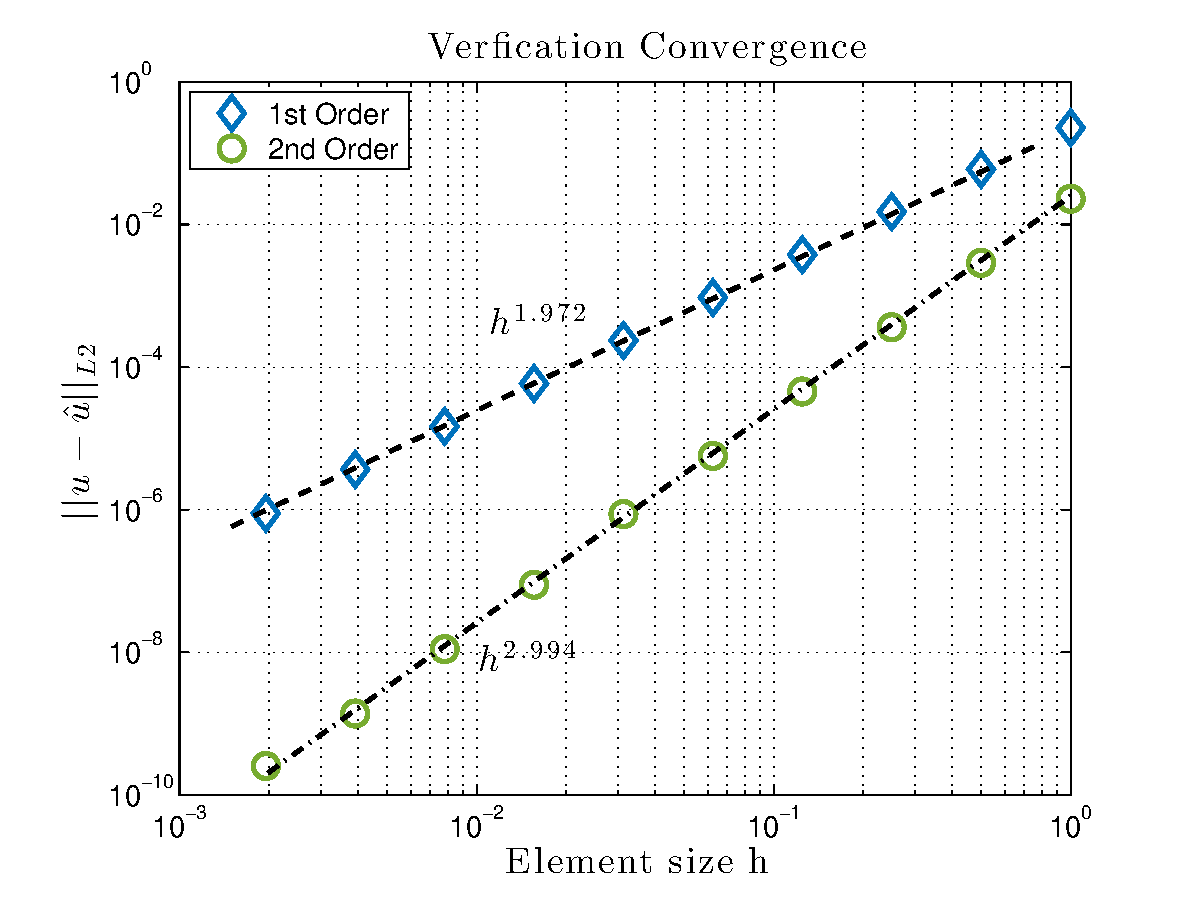
\includegraphics[width=4in]{convergence.eps} 
   \caption{Convergence of 1st and 2nd order elements to the MASA manufactured solution}
   \label{fig:convergence}
\end{figure}

\begin{figure}[H] %  figure placement: here, top, bottom, or page
   \centering
   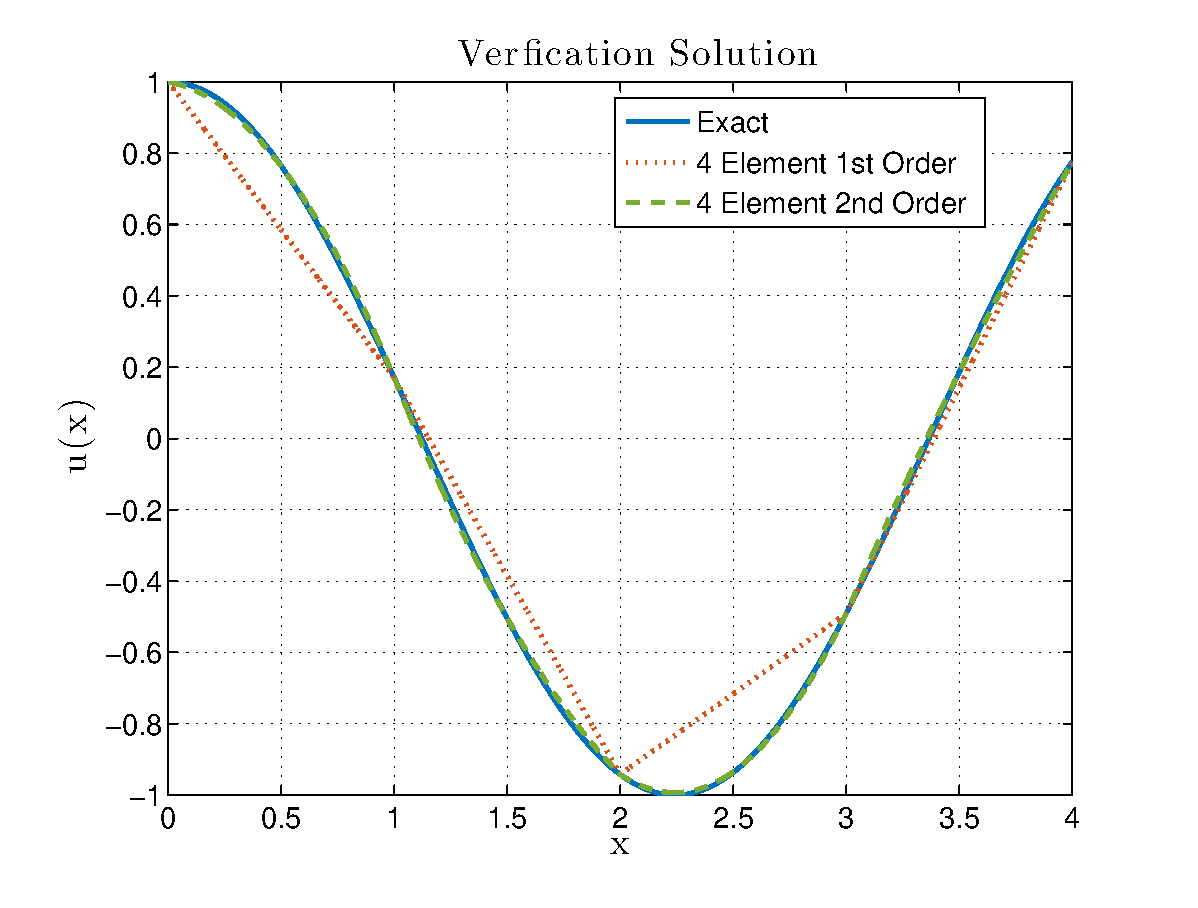
\includegraphics[width=4in]{interpolation.eps} 
   \caption{Interpolation of the MASA exact solution by 1st and 2nd order elements}
   \label{fig:interpolation}
\end{figure}

Figure \ref{fig:timing} shows the comparison of the time spent in the Gauss-Seidel solver vs. the time spent running other parts of the program.  It is clear that the program runtime is dominated by the solution of the linear system.  Figure \ref{sub_timing} shows the breakdown of time spent in other parts of the program.  Most of the time is spent in initialization which includes parsing the input file and allocating memory to Domain and Solver objects.  Building the elements is next, followed by the process of calculating the integrals and inserting them into their global locations.

\begin{figure}[!htbp] %  figure placement: here, top, bottom, or page
   \centering
   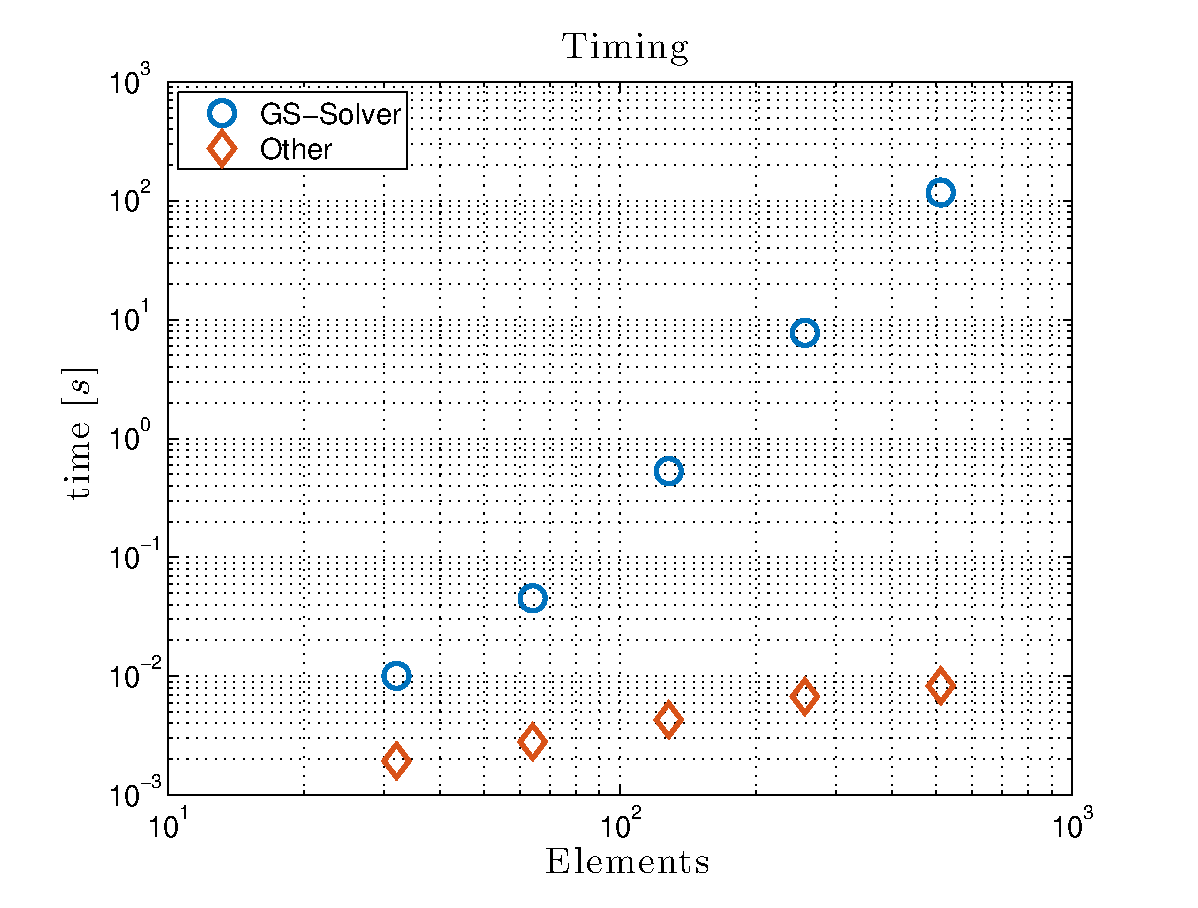
\includegraphics[width=4in]{timing.eps} 
   \caption{Timing compariSson between solver iterations and other program routines}
   \label{fig:timing}
\end{figure}

\begin{figure}[H] %  figure placement: here, top, bottom, or page
   \centering
   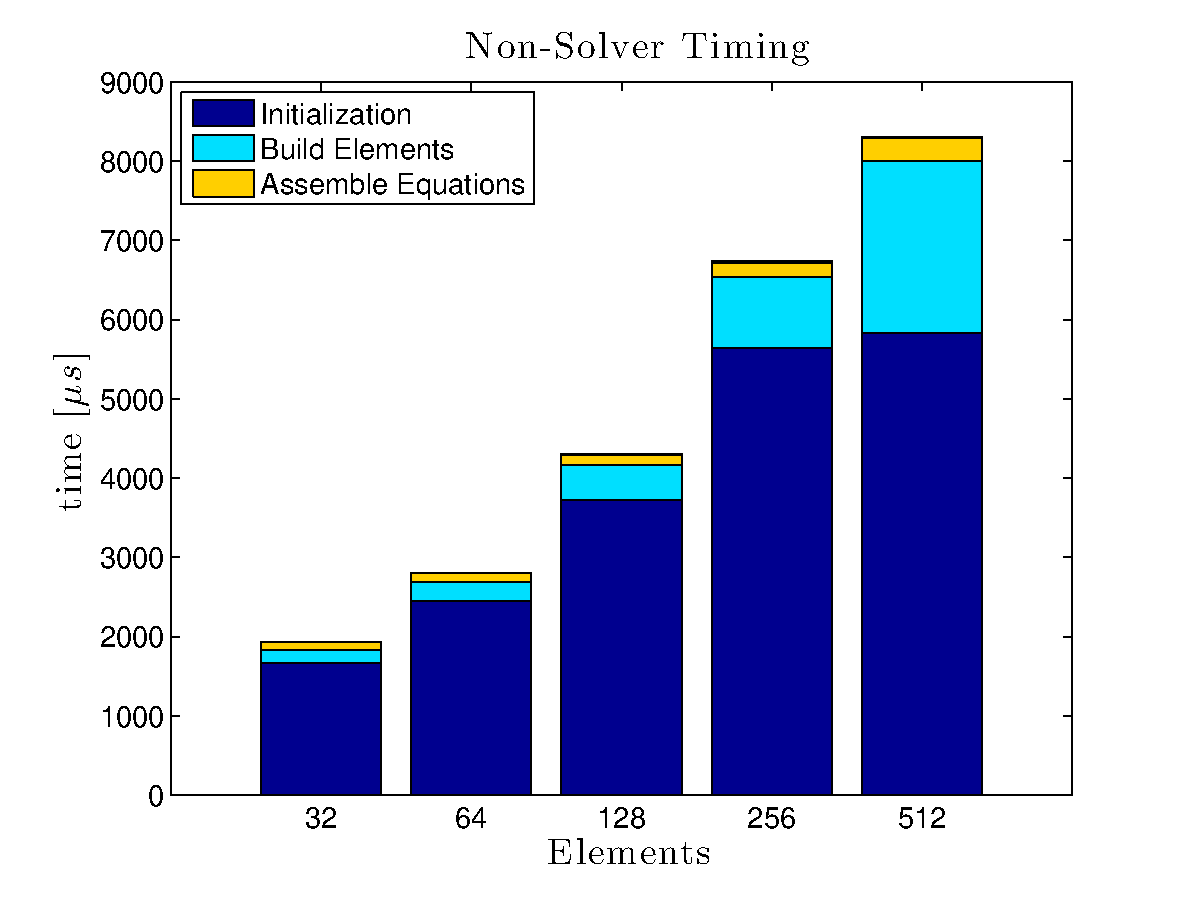
\includegraphics[width=4in]{other_timing.eps} 
   \caption{Timing breakdown for non-solver program components}
   \label{fig:int_error}
\end{figure}

Figure \ref{fig:solvers} shows the comparison of the Jacobi and Gauss-Seidel solver convergence rates for a 1st order element problem.  Here we see that the Gauss-Seidel solver converges in few iterations, although overall solution time is similar between the two.  The jacobi solver does not converge for the second order elements due to lack of diagonal dominance, as shown in the sparsity patter in figure \ref{fig:sparsity}.  Note that with a node renumbering scheme the second order matrix should have a single band for this first order problem.  The Eigen routines available to the user, HouseHolder pivoting and Conjugate Gradient, show a large speedup compared to the hand coded iterative methods.

\begin{figure}[!htbp] %  figure placement: here, top, bottom, or page
   \centering
   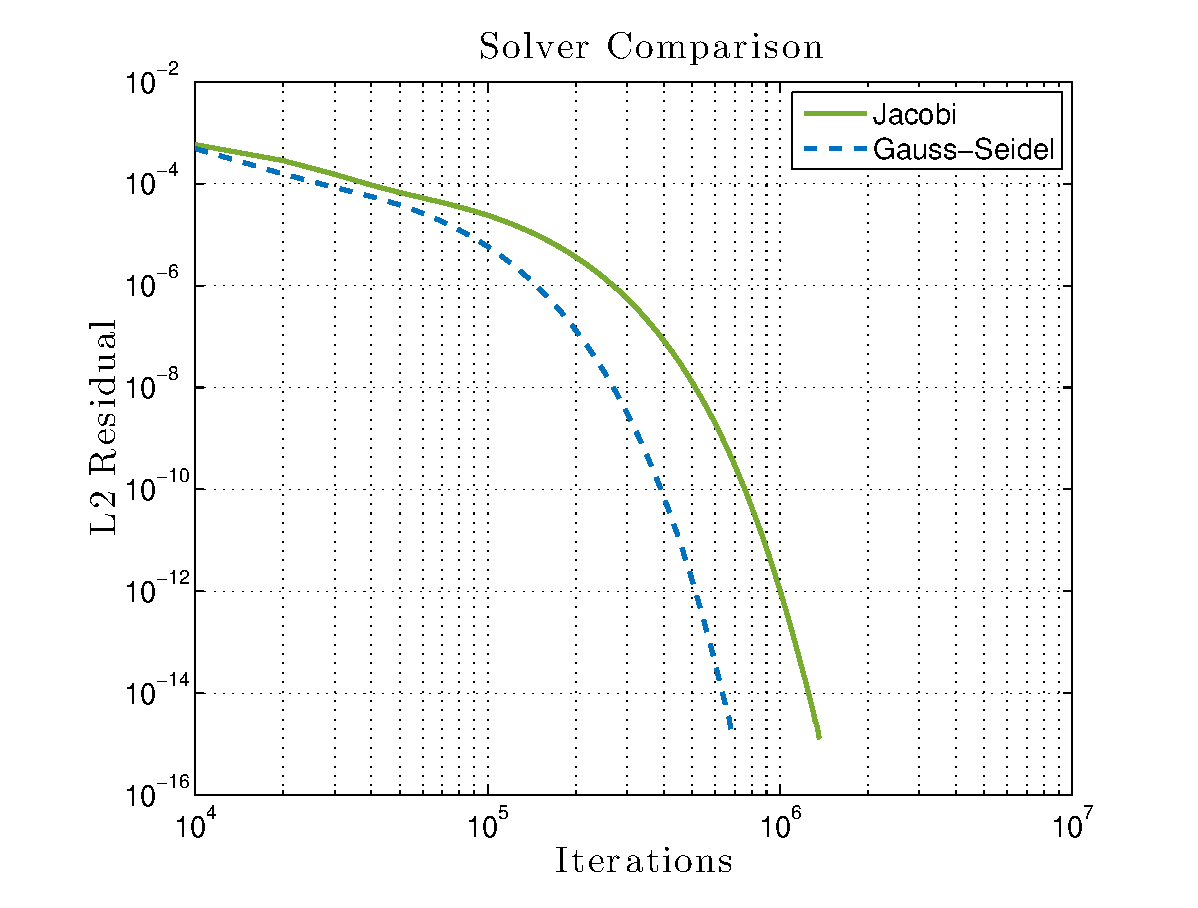
\includegraphics[width=4in]{solver_convergence.eps} 
   \caption{Relative error vs. number of elements}
   \label{fig:solvers}
\end{figure}

\begin{figure}[!htbp] %  figure placement: here, top, bottom, or page
   \centering
   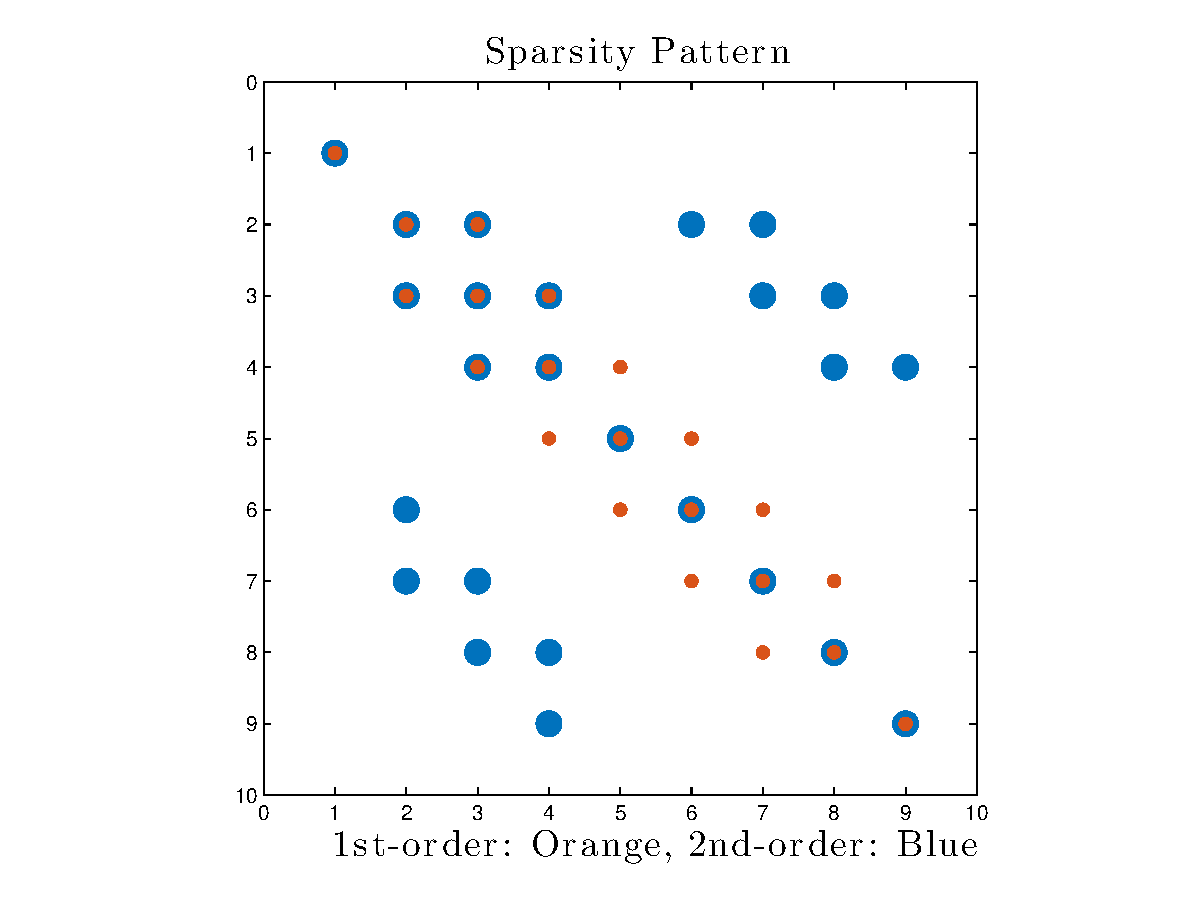
\includegraphics[width=4in]{sparsity.eps} 
   \caption{Relative error vs. number of elements}
   \label{fig:sparsity}
\end{figure}

\section*{Conclusions}

A finite element solver for the steady 1D heat equation was implemented in C++.  External libraries used included Catch for unit testing, Eigen for vector math, GRVY for input parsing and timing, and MASA for manufactured solutions.  The code was verified through a combination of unit tests, as well as tests against MASA analytical solutions.  The code is object oriented and modular which should allow for easy expansion to higher dimensions or unsteady problems.

Overall I am very happy with the outcome of the project and this class.  I was exposed to many ideas techniques and technologies that were completely new to me including: linux and the command line, git based version control, making and building compiled code, unit testing frameworks, object oriented programming, and manufactured solutions.  I feel that I have gained the foundations of a skill set that, even as an experimentalist, will be useful and, with some work, maybe even marketable in the future.

\bibliography{bibliography}
\bibliographystyle{aiaa}
 
\end{document}